\subsection{Diagrammi delle classi del ViewModel}
\subsubsection{Package Controllers}
\begin{figure}[h!]
	\begin{center}
		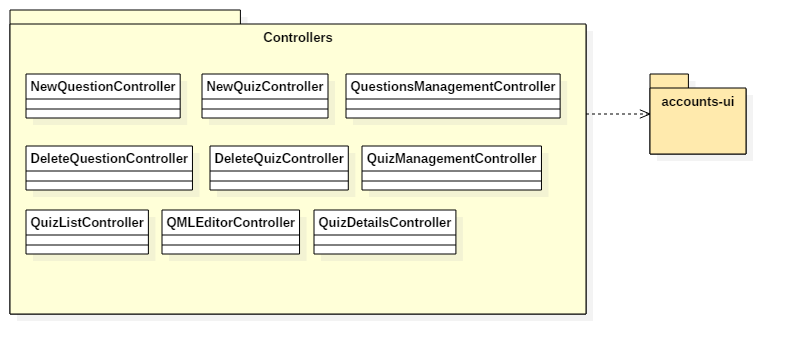
\includegraphics[scale=0.6]{../images/ControllersClass.png}
		\caption{Diagramma delle classi del package Controllers}
	\end{center}
\end{figure}

\subsubsubsection{Classe NewQuestionController}

\begin{itemize}
	\item\textbf{Funzione del componente}: la classe permette di gestire la creazione di una nuova domanda;
	\item\textbf{Relazione d'uso di altre componenti}: il controller è collegato al template QuestionForm.
	\item\textbf{Attività svolte e dati trattati}: Fornisce le funzionalità per la creazione di una domanda, quali la scelta della categoria e l'inserimento del testo, e espone la funzione di salvataggio dei dati inseriti che compongono la nuova domanda.
\end{itemize}

\subsubsubsection{Classe NewQuizController}

\begin{itemize}
	\item\textbf{Funzione del componente}: la classe permette di gestire la creazione di un nuovo quiz (questionario); 
	\item\textbf{Relazione d'uso di altre componenti}: il controller è collegato al template QuizCreationForm;
	\item\textbf{Attività svolte e dati trattati}: fornisce le funzionalità per la creazione del nuovo quiz, tramite la scelta di più domande e la scelta della categoria. Espone la funzione di salvataggio del nuovo quiz.
\end{itemize}

\subsubsubsection{Classe QuizListController}

\begin{itemize}
	\item\textbf{Funzione del componente}:  la classe permette il caricamento e la visualizzazione della lista di quiz disponibili nel sistema;
	\item\textbf{Relazione d'uso di altre componenti}: il controller è collegato al template QuizList;
	\item\textbf{Attività svolte e dati trattati}: la classe si occupa di caricare la lista aggiornata dei quiz creati dagli utenti, e fornisce funzionalità di ordinamento della stessa e di selezione dei singoli quiz per la visualizzazione dei dettagli. 
\end{itemize}

\subsubsubsection{Classe QuizDetailsController}

\begin{itemize}
	\item\textbf{Funzione del componente}: la classe permette di visualizzare le informazioni generali di un quiz, una volta selezionato dalla lista dei quiz;
	\item\textbf{Relazione d'uso di altre componenti}: il controller è collegato al template Quiz. Si relaziona inoltre con il modulo QuizList.
	\item\textbf{Attività svolte e dati trattati}: la classe si occupa di recuperare e rendere visualizzabili le informazioni relative ad un singolo quiz.
\end{itemize}

\subsubsubsection{Classe DeleteQuestionController}

\begin{itemize}
	\item\textbf{Funzione del componente}: la classe fornisce le funzionalità necessarie alla cancellazione di una domanda precedentemente creata;
	\item\textbf{Relazione d'uso di altre componenti}: il controller è collegato al template QuestionList. Si relaziona inoltre con il package Methods.
	\item\textbf{Attività svolte e dati trattati}: la classe si occupa di richiedere la cancellazione di una domanda, precedentemente creata dall'utente, dal sistema.
\end{itemize}

\subsubsubsection{Classe DeleteQuizController}

\begin{itemize}
	\item\textbf{Funzione del componente}: la classe fornisce le funzionalità necessarie alla cancellazione di un quiz precedentemente creato;
	\item\textbf{Relazione d'uso di altre componenti}: il controller è collegato al template QuizList. Si relaziona inoltre con il package Methods.
	\item\textbf{Attività svolte e dati trattati}:  la classe si occupa di richiedere la cancellazione di un quiz, precedentemente creato dall'utente, dal sistema.
\end{itemize}

\subsubsubsection{Classe QuizManagementController}

\begin{itemize}
	\item\textbf{Funzione del componente}: la classe permette di gestire la somministrazione di un questionario;
	\item\textbf{Relazione d'uso di altre componenti}: il controller è collegato al template QuestionCompilation;
	\item\textbf{Attività svolte e dati trattati}: la classe si occupa di gestire la risoluzione di un questionario da parte di un utente fornendo la possibilità di navigare tra le domande, salvando le risposte dell'utente e gestendo il tempo limite. Espone la funzione di consegna del quiz compilato.
\end{itemize}

\subsubsubsection{Classe QuestionsManagementController}

\begin{itemize}
	\item\textbf{Funzione del componente}: la classe permette di gestire la somministrazione di una singola domanda all'interno di un questionario;
	\item\textbf{Relazione d'uso di altre componenti}: il controller è collegato al template Question.
	\item\textbf{Attività svolte e dati trattati}: la classe si occupa di recuperare i dati associati ad una singola domanda di un questionario e di presentarli all'utente. Tali operazioni si svolgono durante la somministrazione all'utente di un questionario.
\end{itemize}

\subsubsubsection{Classe QMLEditorController}

\begin{itemize}
	\item\textbf{Funzione del componente}: fornisce le funzionalità per creare e modificare una domanda tramite editor QML;
	\item\textbf{Relazione d'uso di altre componenti}: il controller è collegato al template QuizCreationForm.
	\item\textbf{Attività svolte e dati trattati}: la classe definisce la logica dello strumento principale di creazione delle domande, l'editor QML, gestisce il testo che viene inserito e espone la funzionalità di checking sintattico del testo inserito.
\end{itemize}

\subsubsection{Package Subscribers}
\begin{figure}[h!]
\begin{center}
	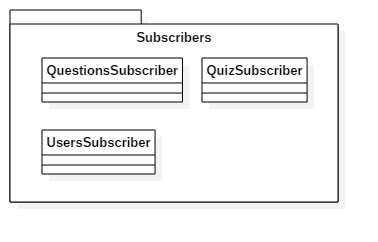
\includegraphics[scale=0.65]{../images/SubscribersClass.png}
	\caption{Diagramma delle classi del package Subscribers}
\end{center}
\end{figure}

\subsubsubsection{Classe QuestionsSubscriber}

\begin{itemize}
	\item\textbf{Funzione del componente}: la classe è necessaria ad effettuare il \emph{subscribe} relativo alla collezione di domande del sistema;
	\item\textbf{Relazione d'uso di altre componenti}: si relazione con la componente QuestionsManagementController;
	\item\textbf{Attività svolte e dati trattati}: la classe espone le funzionalità necessarie ad effettuare il subscribing di una componente del client alla collezione di domande del sistema, se questa è stata precedentemente pubblicata dal server.
\end{itemize}

\subsubsubsection{Classe QuizSubscriber}

\begin{itemize}
	\item\textbf{Funzione del componente}: la classe è necessaria ad effettuare il \emph{subscribe} relativo alla collezione di quiz del sistema;
	\item\textbf{Relazione d'uso di altre componenti}: si relazione con le componenti QuizListController e QuizManagementController;
	\item\textbf{Attività svolte e dati trattati}: la classe espone le funzionalità necessarie ad effettuare il subscribing di una componente del client alla collezione di quiz del sistema, se questa è stata precedentemente pubblicata dal server.
\end{itemize}

\subsubsubsection{Classe UsersSubscriber}

\begin{itemize}
	\item\textbf{Funzione del componente}: la classe è necessaria ad effettuare il \emph{subscribe} relativo alla collezione di utenti del sistema;
	\item\textbf{Relazione d'uso di altre componenti}: si relaziona con il package esterno 'accounts-ui';
	\item\textbf{Attività svolte e dati trattati}: la classe espone le funzionalità necessarie ad effettuare il subscribing di una componente del client alla collezione di utenti del sistema, se questa è stata precedentemente pubblicata dal server.
\end{itemize}

\subsubsection{Package Methods}
\begin{figure}[h!]
\begin{center}
	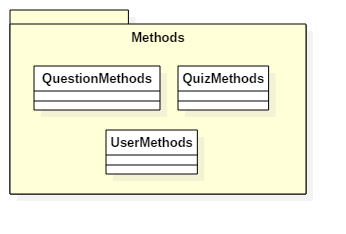
\includegraphics[scale=0.65]{../images/MethodsClass.png}
	\caption{Diagramma delle classi del package Methods}
\end{center}
\end{figure}

\subsubsubsection{Classe QuestionMethods}
\begin{itemize}
	\item\textbf{Funzione del componente}: permette al client di richiedere la modifica della collezione di domande del server;
	\item\textbf{Relazione d'uso di altre componenti}: si relaziona con le classi NewQuestionController e DeleteQuestionController;
	\item\textbf{Attività svolte e dati trattati}: espone le funzionalità di salvataggio e cancellazione di domande dal sistema.
\end{itemize}

\subsubsubsection{Classe QuizMethods}
\begin{itemize}
	\item\textbf{Funzione del componente}: permette al client di richiedere la modifica della collezione di quiz del server;
	\item\textbf{Relazione d'uso di altre componenti}: si relaziona con le classi NewQuizController e DeleteQuizController;
	\item\textbf{Attività svolte e dati trattati}: espone le funzionalità di salvataggio e cancellazione di quiz dal sistema.
\end{itemize}

\subsubsubsection{Classe UserMethods}
\begin{itemize}
	\item\textbf{Funzione del componente}: permette al client di richiedere la modifica della collezione di utenti del server;
	\item\textbf{Relazione d'uso di altre componenti}:  si relaziona con il package esterno 'accounts-ui';
	\item\textbf{Attività svolte e dati trattati}: espone le funzionalità di salvataggio e cancellazione di utenti dal sistema.
\end{itemize}
\newpage			

\subsubsection{Package Interpreter}
\begin{figure}[h!]
\begin{center}
	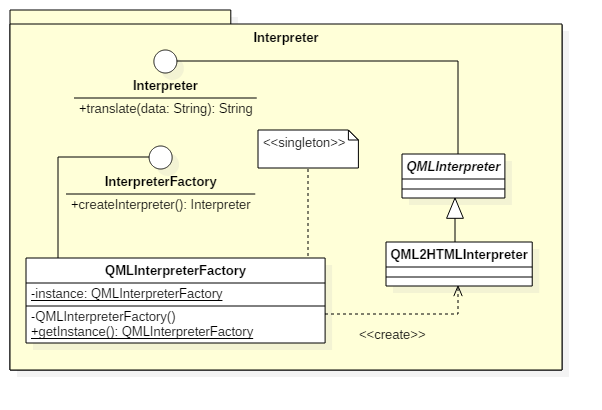
\includegraphics[scale=0.65]{../images/InterpreterClass.png}
	\caption{Diagramma delle classi del package Interpreter}
\end{center}
\end{figure}
\subsubsubsection{Interfaccia Interpreter}
\begin{itemize}
	\item\textbf{Funzione del componente}: interfaccia di base del tipo Interpreter.
	\item\textbf{Relazione d'uso di altre componenti}: può essere concretizzata in diversi tipi di Interpreter.
	\item\textbf{Attività svolte e dati trattati}: definisce il contratto degli Interpreter, cioè le operazioni di traduzione che saranno definite in ogni concretizzazione.
\end{itemize}
\subsubsubsection{Interfaccia InterpreterFactory}
\begin{itemize}
	\item\textbf{Funzione del componente}: interfaccia di base delle Factory di tipi Interpreter.
	\item\textbf{Relazione d'uso di altre componenti}: può essere concretizzata in diversi tipi di InterpreterFactory.
	\item\textbf{Attività svolte e dati trattati}: definisce il contratto delle factory, cioè le operazioni di costruzione di Interpreter che saranno definite in ogni concretizzazione.
\end{itemize}
\subsubsubsection{Classe QMLInterpreterFactory}
La classe QMLInterpreterFactory è un \emph{singleton}.
\begin{itemize}
	\item\textbf{Funzione del componente}: crea oggetti di tipo QMLInterpreter.
	\item\textbf{Relazione d'uso di altre componenti}: è concretizzazione della classe InterpreterFactory. Crea oggetti QMLInterpreter.
	\item\textbf{Attività svolte e dati trattati}: crea su richiesta oggetti di tipo QMLInterpreter.
\end{itemize}
\subsubsubsection{Classe QMLInterpreter}
\begin{itemize}
	\item\textbf{Funzione del componente}: classe astratta che rappresenta gli Interpreter che traducono codice QML in un altro formato.
	\item\textbf{Relazione d'uso di altre componenti}: è sottotipo di Interpreter. Può essere concretizzata in più tipi di QMLInterpreter.
	\item\textbf{Attività svolte e dati trattati}: definisce il contratto dei QMLInterpreter, cioè le operazioni di traduzione da QML verso altri linguaggi.
\end{itemize}
\subsubsubsection{Classe QML2HTMLInterpreter}	
\begin{itemize}
	\item\textbf{Funzione del componente}: traduce codice QML in codice HTML.
	\item\textbf{Relazione d'uso di altre componenti}: è concretizzazione di QMLInterpreter.
	\item\textbf{Attività svolte e dati trattati}: riceve in input domande in QML e le traduce in codice HTML visualizzabile da browser.
\end{itemize}

\subsubsection{Classe Router}
\begin{figure}[h!]
\begin{center}
	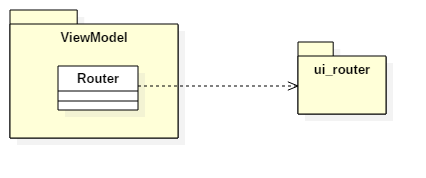
\includegraphics[scale=0.65]{../images/Router.png}
	\caption{Diagramma della classe Router}
\end{center}
\end{figure}
\begin{itemize}
	\item\textbf{Funzione del componente}: implementa il routing dinamico dell'applicazione. Permette di dividere la parte statica dell'applicazione dalla parte che va caricata dinamicamente;
	\item\textbf{Relazione d'uso di altre componenti}: Utilizza il package esterno ui-router. Conosce i Template dell'applicazione.
	\item\textbf{Attività svolte e dati trattati}: il Router collega elementi di navigazione associando Url univoci al caricamento dinamico di specifici template.

\end{itemize}

\newpage